\section{Experiments for model validation}
\label{experiments}

In this section, we carried out a number of experiments in order to validate the radio model. 

All the experiments were carried using LAUNCHXL-CC1350-4 evaluation boards with CC1350 RF microcontrollers 
by Texas Instruments. We used a quiet frequency in the 434~MHz band, for which the boards are designed,
and we used the built-in helix antenna printed on the boards. This antenna is fairly inefficient, resulting
in about 4x to 8x degradation in communication range. We used it because the shorter 
ranges make testing easier
and also because antennas on small wildlife tags also tend to be inefficient due to the tiny ground plane.
The chips that we tested are widely-used in miniature wildlife tags, and they essentially represent a modern
version of the chips that were used on the original Encounternet tags.
% requires more citations.

In all tests we configured the radios for GFSK modulation, 500~kb/s, $\pm 250$~kHz deviation, 1243~kHz receive bandwidth,
and 10~dBm transmit power. We used a Windows program called SmartRF Studio version~7 to drive the boards during
the tests and to log received packets. In all tests one board transmitted one 1.87~packets per second (intervals of
500~ms between packets). Packets consisted of a 4-byte preamble, 4-byte sync workd, a length byte, 30-byte payload 
that includes a sequence number, and a 2-byte checksum. The fast transmission rate reduces power consumption (per byte and
per packet) and leads to short communication ranges, which are consistent with the goal of registering close encounters.

In a preliminary test, we configured one board to transmit packets, one board to receive them, and a third to transmit a 
CW carrier at the same frequency. The three boards were at distances of 0.4~m from each other. When the CW transmitter
was off, virtually all packets were received correctly. When the CW transmitter was on, virtually no packets were received.
This verifies that interference indeed blocks the receiver and may prevent packets from being received.
% It would have been good to transmit two packets simulteneously but there is no easy way to synchronize the boards.

\begin{figure}[h]
    \centering
    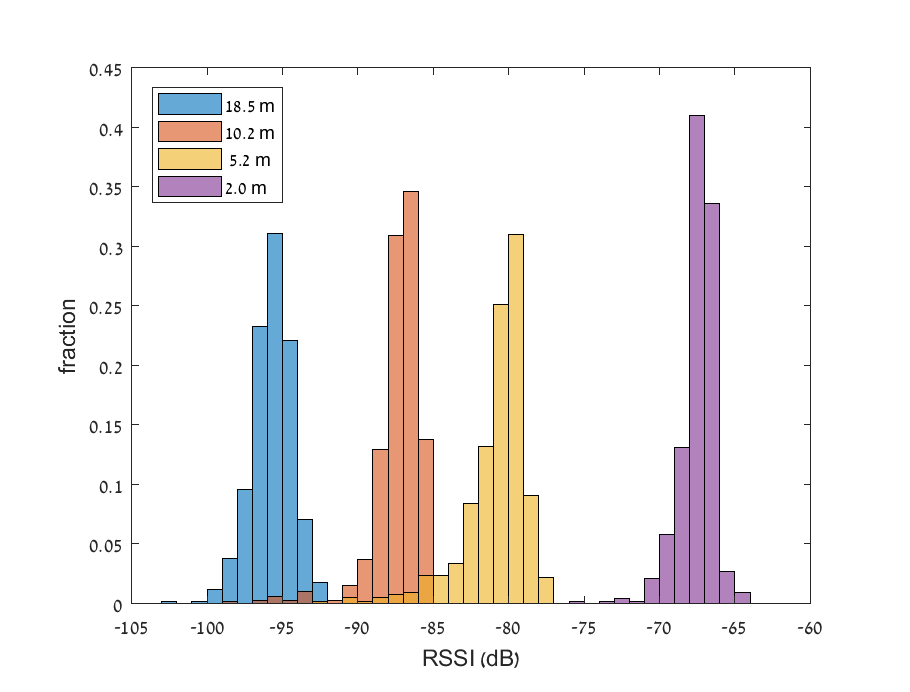
\includegraphics[width=3in]{experiments/rssiHistograms.eps}
    \caption{Histograms of the RSSI of received packets at different distances between 
    the transmitter and the receiver. At the four distances reported in the figure, 
    virtually all transmitted packets were received correctly.}
    \label{fig:rssiHistograms}
\end{figure}

\begin{figure}[h]
    \centering
    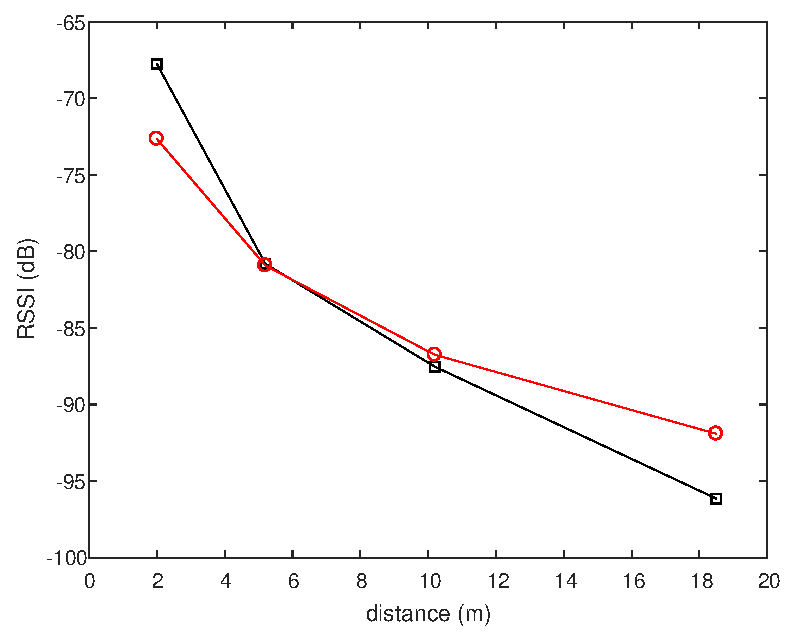
\includegraphics[width=3in]{experiments/rssiDistance.eps}
    \caption{Mean RSSI (after removal of outliers) at different distances, in black. 
    The red curve is a least-square
    fitting of the data to a 6~dB attenuation when the distance doubles.
    The means shown in this figure are of the center 50\% of the packets; 
    the extreme 50\% were filtered to remove outliers.}
    \label{fig:rssiDistance}
\end{figure}

In the main test, we placed the transmitter board at a fixed position, about 1.4~m above ground, and measured receive
performance at various distances between 2 and 78~m in an outdoor area with some human activity (but not much). We 
maintained each test position for at least 5 minutes.
The receiver board was also placed about 1.4~m above ground. In all the tests shown in graphs the transmit
and receive antennas were pointed at each other. We also performed a few tests with the receive antenna rotated 90~degrees;
RSSI values were about 1--2~dB lower but the overall results were similar; this is consistent with the characterization
of the antenna, which indicates that it is fairly omnidirectional.
The main results are shown in Figure~\ref{fig:rssiHistograms}.
At each distance we measured the fraction of correctly-received packets and the RSSI of each packet. At the four
distances reported in the figure, virtually all transmitted packets were received correctly. We can see a clear
statistical correlation between distance and RSSI. Figure~\ref{fig:rssiDistance} shows that the RSSI values
roughly follow the theoretical rule that stipulates a 6~dB attenuation when the distance doubles. The means
shown in this figure are of the center 50\% of the packets; the extreme 50\% were filtered to remove outliers.

We also tested performance at distances of 53~m and 78~m. At these distances, results were inconsistent. In one test
at 78~m, 84\% of the packets with mean RSSI of -98~dB. But in another test two hours later, only 2\% of the packets
were correctly received. At 53~m, no packets were received correctly for over 5 minutes. This location was in a depression,
about 3~m lower than both the transmitter and from the 78~m position; this may have contributed to the worse performance.
The main conclusion from these long-distance experiments (long given the bit rate) is that packets can sometimes be received
at fairly long distances and with RSSI values that typically characterize much shorter distances. 

However, the results also indicate that by dropping packets with low RSSI, say below -90~dB for these settings, we can
effectively limit the communication range to 20~m or so.


\section{Simulations for protocol validation}
\label{Simulations}

In this section,  
we evaluate the performance of our protocol by extensive simulations, 
and results show our protocol achieves good scalability. 
We also modeled the mobility and herd characteristics of wild animals,
and results validate the efficiency of our protocol.


\subsection{Parameter Setting}

To conduct the simulation tests, we carried out some pre-tests to determine the 
parameters of our protocol.
We selected the appropriate values and fixed the parameters as Table~\ref{para}.

\begin{table}[htbp]
	\caption{Parameter Settings}
	\label{para}
	\centering
	\scalebox{0.9}{
	\begin{tabular}{|c|c|c|}
		\hline
        \textbf{Notation} & \textbf{value} & \textbf{Description}  \\
        \hline
		\textbf{$2\hat{t_0}$} & \textbf{$20$ $ms$} & \makecell[l]{The time length of a synchronized slot in reality.}\\
        \hline
        \textbf{$D$} & \textbf{$20$ $m$} & \makecell[l]{The radio range of tags.}\\
		\hline
		\textbf{$\omega_0$} & \textbf{$0.5$} & \makecell[l]{Fixed transmitting probability in Detecting Stage.}\\
        \hline
        \textbf{$\omega_t$} & \textbf{$0.5$} & \makecell[l]{Initial transmitting probability in Connecting Stage.}\\
		\hline
		\textbf{$\zeta$} & \textbf{$0.5$} & \makecell[l]{Upper bound of the transmitting probability in \\ Connecting Stage.} \\
		\hline
		\textbf{$\epsilon$} & \textbf{$1.0$} & \makecell[l]{Adjustment factor in Connecting Stage.} \\
		\hline		
    \end{tabular}
    }
\end{table}

Next, we selected the baseline methods to compare with our protocol. 
Existing methods to encounter registration problem are mainly based on fixed transmitting 
probability~\cite{Menhill2012NovelTelemetry,Rutz2012AutomatedMapping}
(i.e., agents transmit a beacon with a fixed probability $p$ and listen with $1-p$).  
Note that, if $p$ is too large, there would be multiple transmissions in a time slot which results in 
collisions; if $p$ is too small, there would be no transmissions in a time slot which results 
in long latency fot the encounter process.
We tested different values of transmitting probabilities and chose the following three settings for comparison: 
\begin{itemize}
    \item \textbf{Baseline I:} fix the transmission probability as $0.05$. 
    \item \textbf{Baseline II:} fix the transmission probability as $0.1$. 
    \item \textbf{Baseline III:} fix the transmission probability as $0.2$. 
\end{itemize}


\subsection{Scalability}

The number of encounter animals in the wild varies from a handful to hundreds. 
Therefore, scalability is a crucial factor for encounter protocols. 
In our testbed, we simulated a group of agents to evaluate scalability 
regarding agent amount and duty cycle.

\begin{figure}[!h]
    \centering
    \subfigure[]{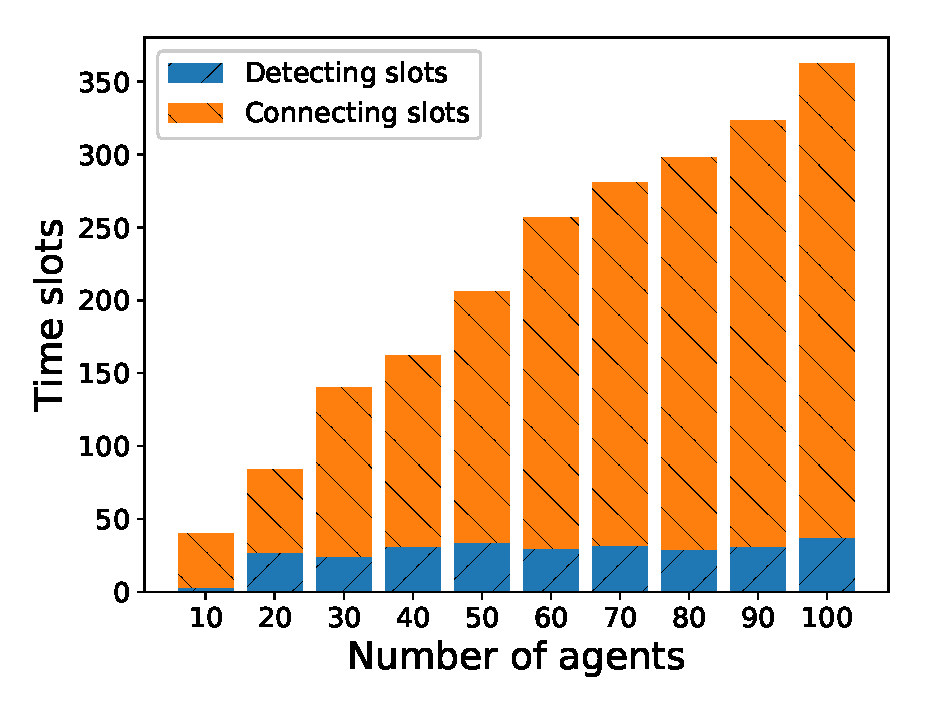
\includegraphics[width=1.65in]{figures/figure1.eps}}
    \hspace{0.01in}
    \subfigure[]{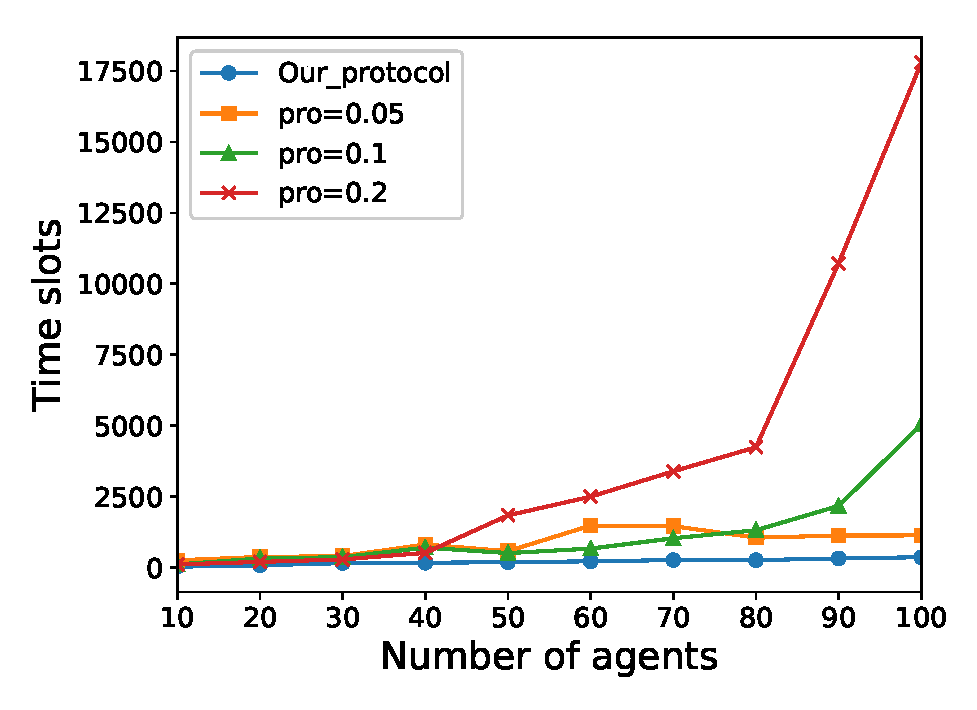
\includegraphics[width=1.65in]{figures/figure3.eps}}
    \caption{Time for encounter process increases when the number of agents grows from $10$ to $100$.
    Figure~(a) depicts the slots for detecting stage and connecting stage of our protocol and figure~(b)
    compares our protocol with the three baseline methods.}
    \label{fig_num}
\end{figure}


In Fig.~\ref{fig_num}, we fix the duty cycle as $0.25$ and 
increase the number of agents from $10$ to $100$.
Fig.~\ref{fig_num}~(a) illustrates that,
the number of slots for the encounter process 
of our protocol grows as the number of agents is ascending. Particularly,
the slots needed in the detecting stage remain steady.
This is because although more agents need to be switched to the connecting stage,
they meanwhile add to the possibility
that an listening agent turn to connecting stage in each time slot.
When compared to the baseline methods as showed in Fig.~\ref{fig_num}~(b), our protocol takes the least latency
to achieve encounter process, and the time of the other three methods increases
markedly as the agent amount grows while that of our protocol still stays in a low lever.

\begin{figure}[!h]
    \centering
    \subfigure[]{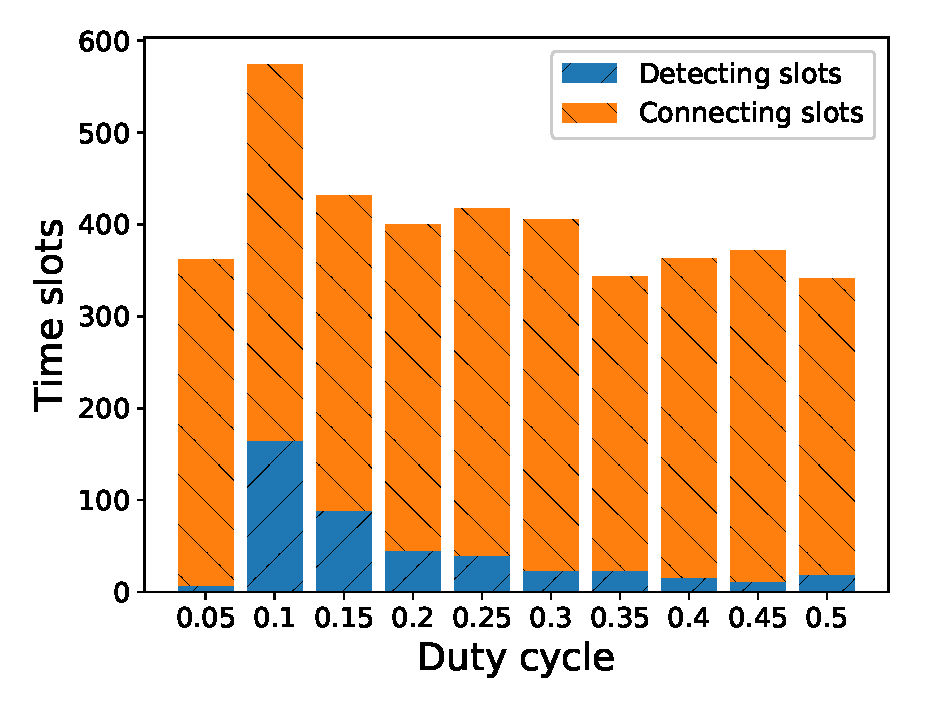
\includegraphics[width=1.65in]{figures/figure2.eps}}
    \hspace{0.01in}
    \subfigure[]{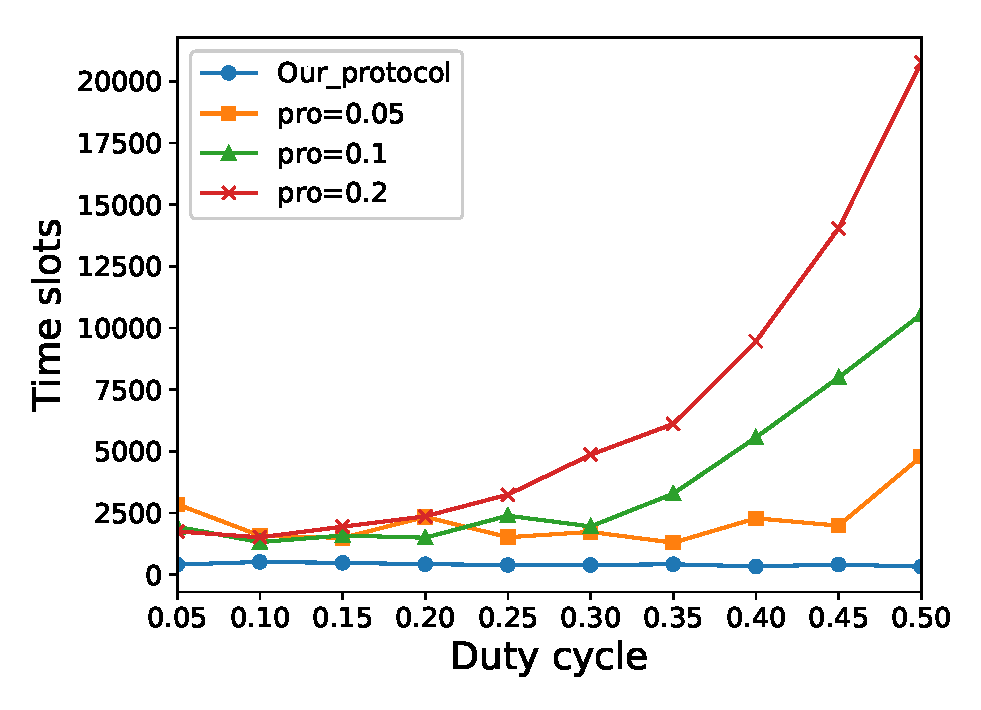
\includegraphics[width=1.65in]{figures/figure4.eps}}
    \caption{Time for encounter process increases when the duty cycle grows from $0.05$ to $0.5$.
    Figure~(a) depicts the slots for detecting stage and connecting stage of our protocol and figure~(b)
    compares our protocol with the three baseline methods.}
    \label{fig_DC}
\end{figure}

In Fig.~\ref{fig_DC}, we fix the the number of agents as $100$ and
increase duty cycle from $0.05$ to $0.5$. Fig.~\ref{fig_DC}~(a) show that
the time for encounter process of our protocol stays steady when duty cycle varies.
Particularly, the slots needed in the detecting stage decreases when duty cycle increases.
This is because higher duty cycle increases the probability that an agent is active in each slot.
Also we see the trend in Fig.~\ref{fig_DC}~(b) that the baseline methods increases the latency as duty cycle rises.

Next, we record the encounter registration rate in each time slot.
Encounter registration rate is defined as the proportion of agents that has been 
recorded. 

\begin{figure}[!h]
    \centering
    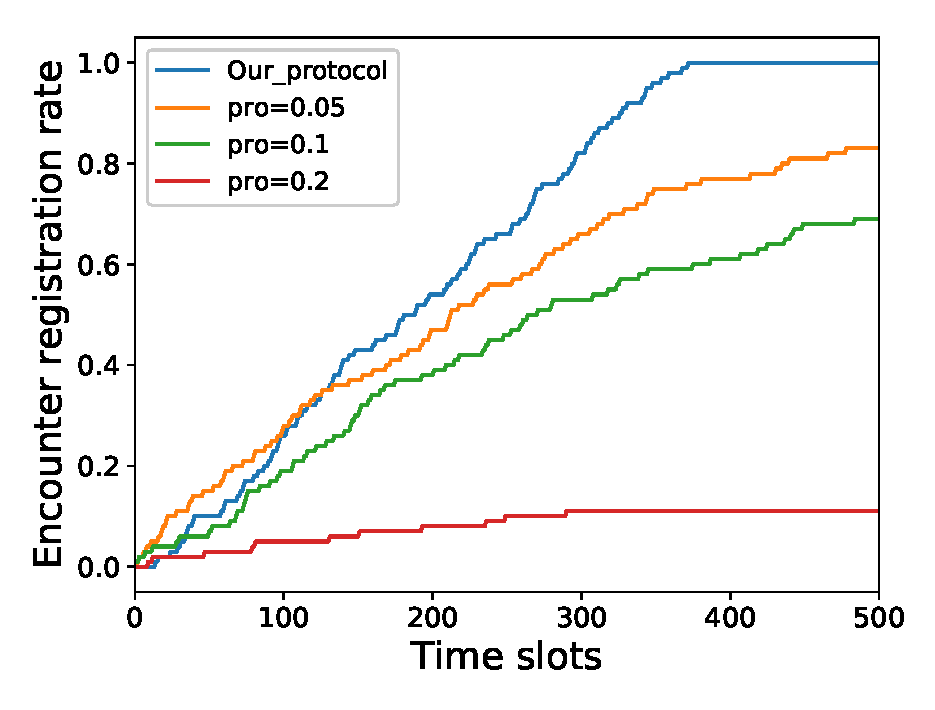
\includegraphics[width=3in]{figures/figure5.eps}
    \caption{Encounter process with $100$ agents and duty cycle of $0.25$. 
    Encounter registration rate increases as time goes on. Our protocol keeps
    the highest rate during the whole process.}
    \label{fig5}
\end{figure}

We set the number of agents as $100$, and fix
duty cycle as $0.25$ in Fig.~\ref{fig5} and $0.5$ in Fig.~\ref{fig6} respectively.
The same trend can be seen that our protocol has higher encounter registration rate
all the time and reaches to $1.0$ faster than other methods.

\begin{figure}[!h]
    \centering
    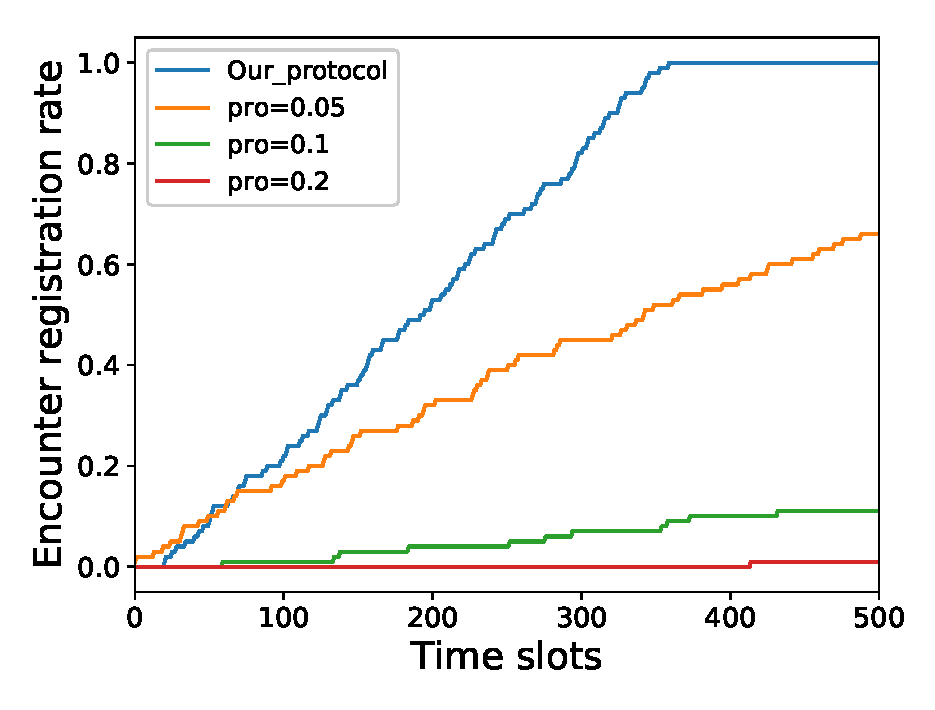
\includegraphics[width=3in]{figures/figure6.eps}
    \caption{Encounter process with $100$ agents and duty cycle of $0.5$. 
    Encounter registration rate increases as time goes on. Our protocol keeps
    the highest rate during the whole process.}
    \label{fig6}
\end{figure}


In conclusion, our protocol outperforms the fixed transmitting probability methods 
and has better scalability. 


\subsection{Mobility}

\begin{figure*}[!t]
    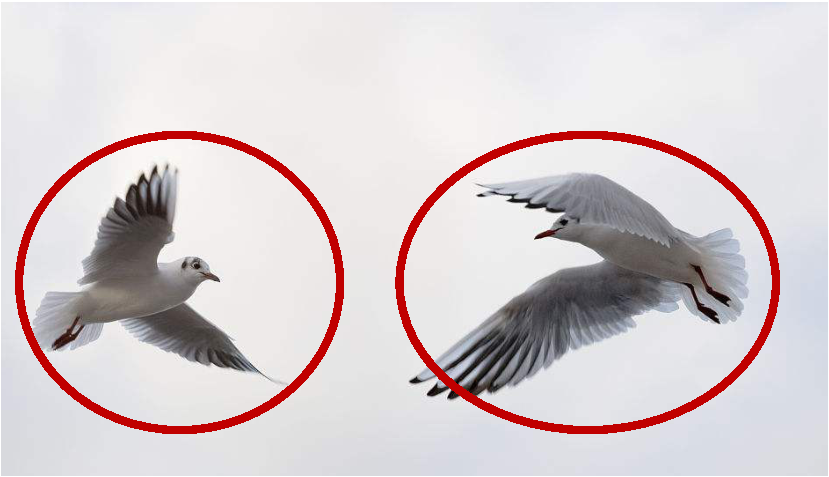
\includegraphics[width=.32\textwidth]{figures/AtoA}
    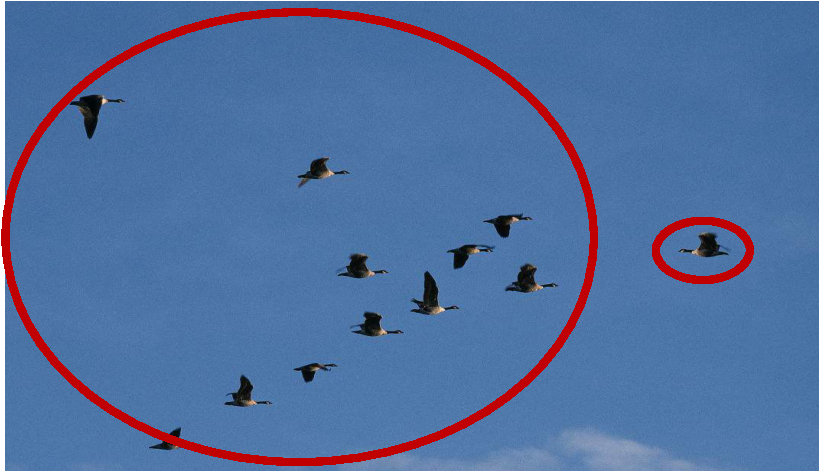
\includegraphics[width=.32\textwidth]{figures/AtoG}
    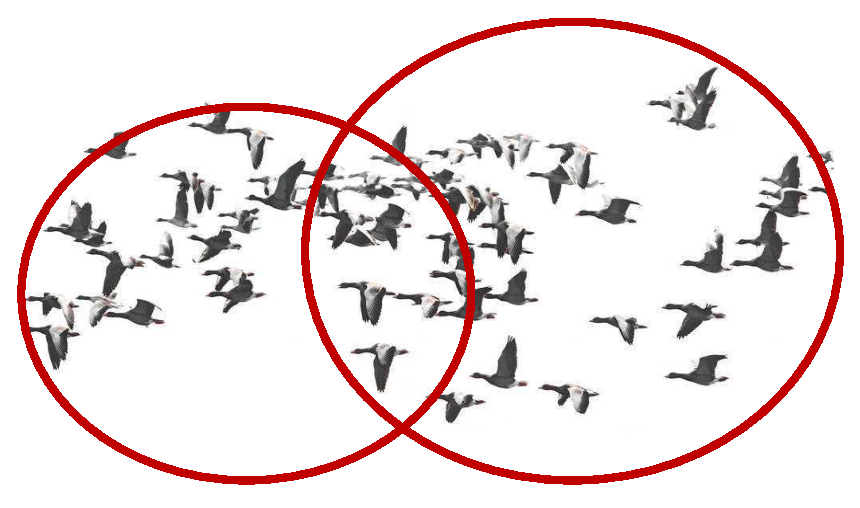
\includegraphics[width=.32\textwidth]{figures/GtoG}
    \caption{Encounter examples of three fundamental cases}
    \label{examples}
\end{figure*}

The essential difference between a wildlife tracing system
and a mobile wireless network is the variability among species in their movement and 
interaction behavior. The key challenge is that depending on targeted animals, 
the moving speed and mobility might vary, and 
the herd characteristics are also different depending on the targeted animals. 

In this paper, we consider three explicit animal models of mobility
and build the simulation models as they relate to animal movement and interaction. 
This is the same approach that has been used in mobile wireless networks where 
human and vehicular mobility are assigned rigorous underpinnings.
Specifically, we model their moving speed as follows:
\begin{itemize}
    \item \textbf{Species I:} move at speed of $50$ m/s. 
    \item \textbf{Species II:} move at speed of $30$ m/s. 
    \item \textbf{Species III:} move at speed of $10$ m/s. 
\end{itemize}
Recall that the time length of a synchronized slot in reality 
is set as $20 ms$ and the radio range is set as $20 m$.

We evaluate our protocol in three simple and heuristic cases, as depicted in Fig.~\ref{examples}.
\begin{itemize}
    \item Case I: encounter for two agents, 
    e.g., two birds fly towards each other and then 
    fly apart, as depicted in Fig.~\ref{examples}~(a). 
    \item Case II: encounter for a single 
    agent with a group of agents, e.g., a bird fly into 
    a group of birds, as depicted in Fig.~\ref{examples}(b).
    \item Case III: encounter for two groups of agents, 
    e.g., two groups of birds fly towards each other and then fly 
    apart, as depicted in Fig.~\ref{examples}(c).
\end{itemize}

\subsubsection{Encounter for two agents}

We can see from Fig.~\ref{fig7} that both
agents conducting our protocol can record each
other regarding all the three species.

\begin{figure}[!h]
    \centering
    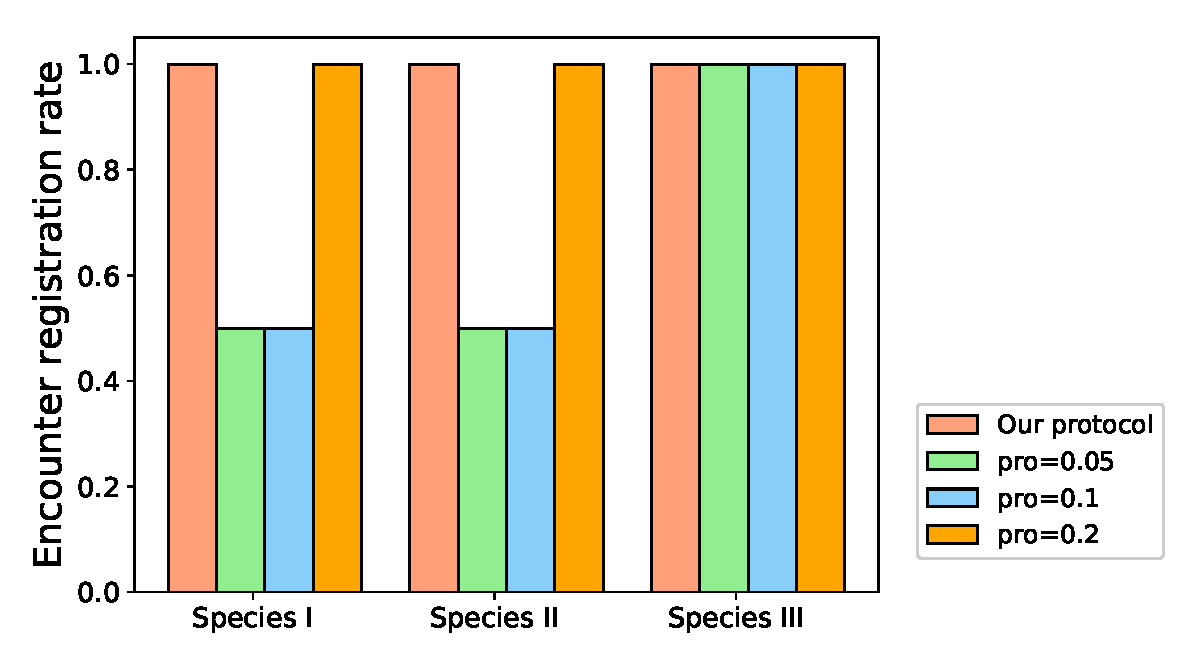
\includegraphics[width=3in]{figures/figure7.eps}
    \caption{Encounter for two agents. Our protocol
    achieves $100\%$ encounter registration rate.}
    \label{fig7}
\end{figure}

\subsubsection{Encounter for a single 
agent with a group of agents}

We can see from Fig.~\ref{fig8} that 
our protocol has higher encounter
registration rate (the proportion of agents can 
be recorded by the single agent) than any other methods.
Particularly, our protocol achieves nearly $100\%$ registration
rate regarding species II and species III.
This is because these two species move slower than species I 
so that agents can be recorded in greater possibilities. 


\begin{figure}[!h]
    \centering
    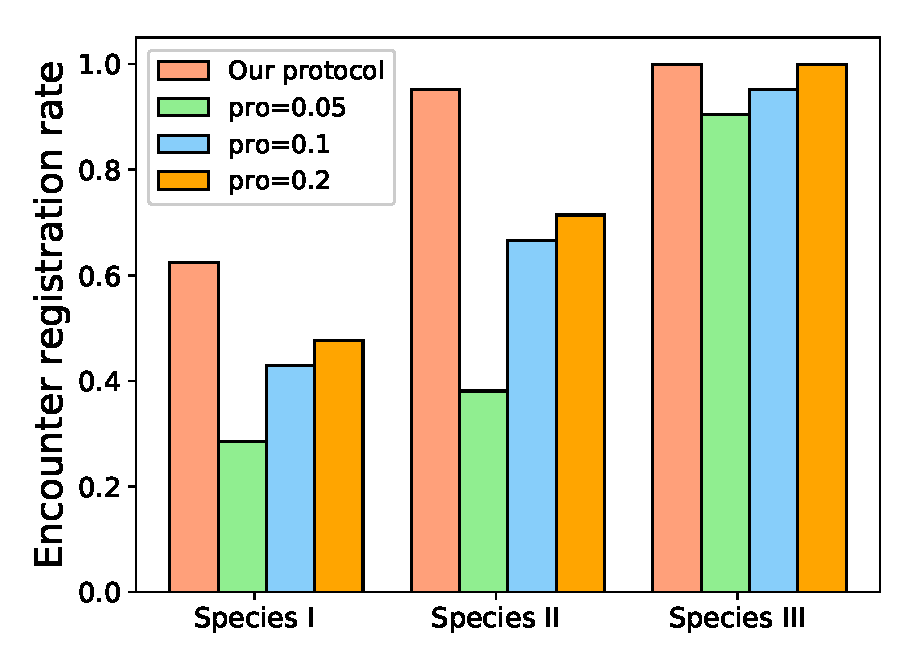
\includegraphics[width=3in]{figures/figure8.eps}
    \caption{Encounter for a single 
    agent with a group of agents. Overall, our protocol
    achieves higher encounter registration rate.}
    \label{fig8}
\end{figure}

\subsubsection{Encounter for two groups of agents}

Fig.~\ref{fig9}~(a) shows the proportion of agents in group A can 
be recorded by the agents in group B, and Fig.~\ref{fig9}~(b) describes
the opposite case. Overall, our protocol achieves higher encounter 
registration rate than any other methods. Particularly, species III
has higher encounter registration rate than species II and species III.
This is because species III moves the most slowly and thus there are more 
chances for agents to detect and connect their peers. 

\begin{figure}[!h]
    \centering
    \subfigure[]{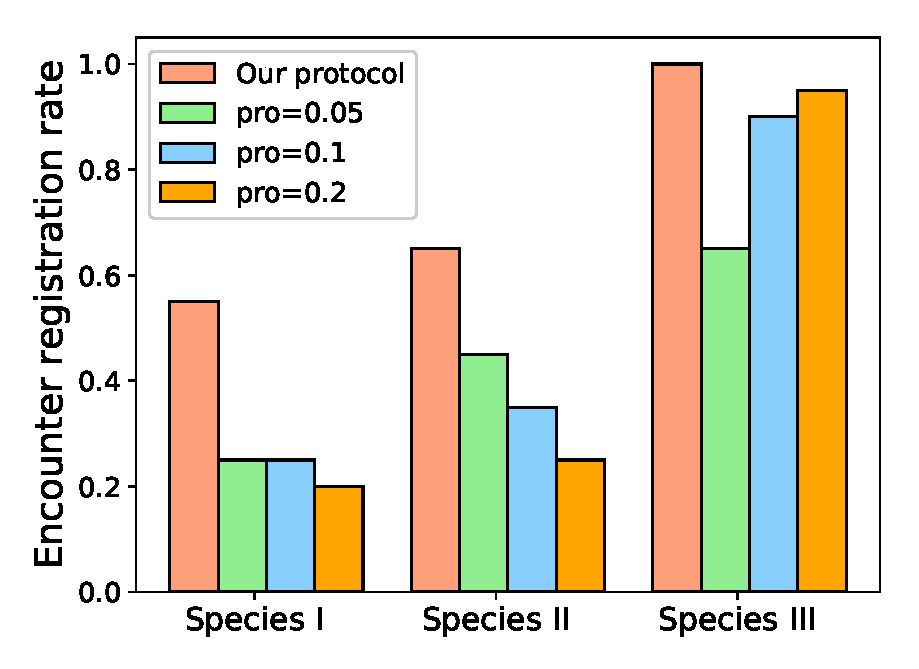
\includegraphics[width=1.65in]{figures/figure9_A.eps}}
    \hspace{0.01in}
    \subfigure[]{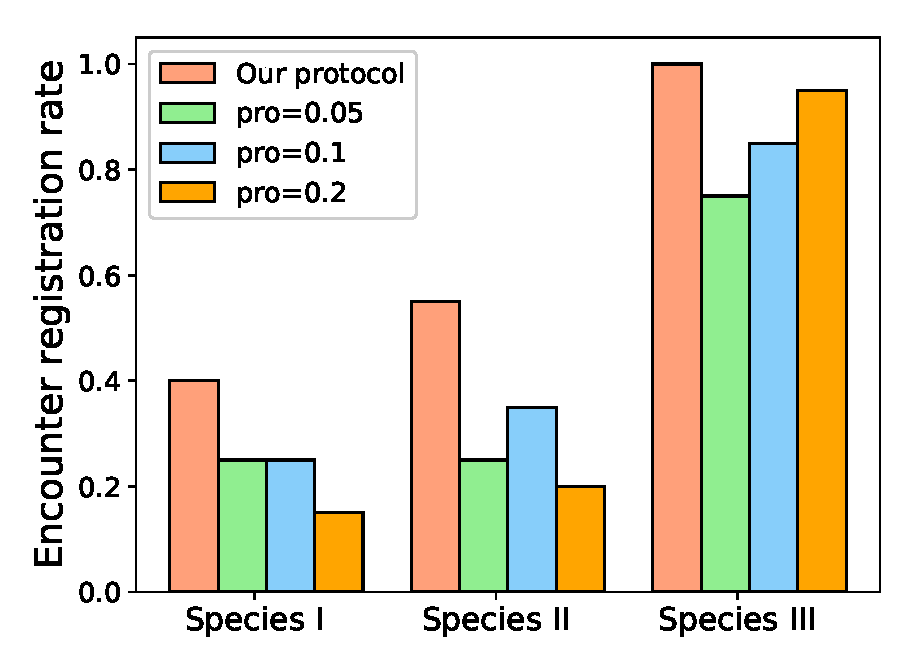
\includegraphics[width=1.65in]{figures/figure9_B.eps}}
    \caption{Figure~(a) shows the proportion of agents in group A can 
    be recorded by the agents in group B, and Figure~(b) describes
    the opposite case. Overall, our protocol
    achieves higher encounter registration rate.}
    \label{fig9}
\end{figure}
